\chapter{A failing direct interpretable reinforcement learning algorithm}
\epigraphhead[30]{\selectlanguage{english}\epigraph{I have not failed. I've
    just found 10.000 ways that won't work.}{Thomas A. Edison}}

\section{Iterative Bounding Markov Decision Processes}
We start by considering a very basic Markov decision process (def) for which we would like decision tree (def) policies. 
 
In 2021, Topin et. al. introduced Iterative Bounding Markov decision process (IBMPD) (cite). It is, to the best of our knowledge, the only work in which decision tree policies are \textit{grown} using the RL object (def).
We insist here on \textit{growing} to refer to trees whose nodes and leaves structure is not knows \textit{a priori} as opposed to parametric trees--trees which structure is fixed-- and can be optimized with the policy gradient theorem (cite).
In supervised learning a similar distinction exists too (cite).

The policy gradient theorem or random search can also be used in to learn linear policies (cite) that should be more interpretable than deep neural netwok. 
In this seminal work Topin et. al., formulate learning a decision tree policy for an MDP as solving an augmented MDP where some actions are adding decision nodes to a tree structure or taking base actions. (figure)
More interestingly, IBMDP can generalize to any sort of tree-like policies where nodes need only to be binary functions of features.  

\section{Litterature and results on POMDPs}
Without mentionning explicitely Topin et.al. propose to learning in IBMDPs by solving a Partially Observable MDP (cite). POMDPs are notorously more difficult to solve than MDPs (cite).
In particular, not all policies for $\mathcal{M}_IB$ are decision tree policies for $\mathcal{M}$. Only policies from partial observation to actions are trees. 
Hence learning a decision tree policy for an MDP can be done by learning a \textit{deterministic} and \textit{reactive} policy for a POMDP. 
In general, this problem cannot be solved exactly with dynamic programming because of intrinsic POMDP limitations described in the work of Michael Littman (cite).

We will show that three of those limitations arise in direct interpretable RL:
\begin{enumerate}
    \item The optimal policy in a POMDP can be stochastic
    \item The optimal policy in a POMDP does not necessarily maximizes all state values simultaneously
    \item Q-Learning like algorithms do not necessirily converge to the optimal Q-values.
\end{enumerate}

In addition to those limitaions that are inherited from POMDPs, IBMDPs bring their own intrinsic challenges:
\begin{enumerate}
    \item The action space might need to be state dependent
    \item It is hard to align RL agents for IBMDPs
\end{enumerate}

\section{IBMDP and Didactic example}
Given an MDP $\mathcal{M}= \langle S, A, R, T, T_0 \rangle$, an Iterative Bounding Markov decision process is defined as follows.
\begin{definition}
    Given an MDP $\mathcal{M}= \langle S, A, R, T, T_0 \rangle$, an Iterative Bounding Markov decision process $\mathcal{M}_{IB}$ is a tuble $\langle S, O, A, A_{IG}, R, \zeta, T, T_0, P\rangle$.
    The IBMDP is an augmented version of an MDP. The states in an IBMPD are concatenations of $s\in S \subset [L_1, U_1]\times\dots \times [L_n, U_n] \subsetneq \mathbb{R}^n$ and bounding values $o = (L_0) \in O$ 
\end{definition}
\subsection{An MDP for which we want a decision tree policy}
(figure) Do figure of POMDP graphical models with grid world. 
We consider a 2×2 grid world Markov Decision Process (MDP) defined as follows:
\begin{itemize}
    \item \textbf{States}: Four cells labeled $S_0$, $S_1$, $S_2$, and $G$ (goal state) arranged in a 2×2 grid.
    \item \textbf{Actions}: At each state, the agent can move right ($\rightarrow$) or down ($\downarrow$) up ($\uparrow$) or left ($\leftarrow$).
    \item \textbf{Transitions}: Movements are deterministic, following the direction of the chosen action. Actions that would lead outside the grid leave the agent in the same state.
    \item \textbf{Rewards}: All transitions yield a reward of 0, except for any action taken from the goal state $G$, which yields a reward of 1.
    \item \textbf{Objective}: Maximize the expected discounted cumulative reward.
\end{itemize}
\begin{figure}[ht]
    \centering
    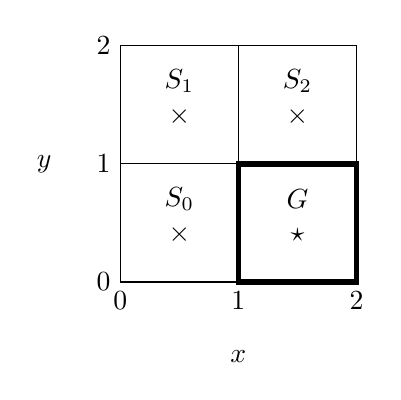
\begin{tikzpicture}[scale=1.5]
        % Draw the grid cells
        \draw (0,0) grid (2,2);
        
        % Add ticks on axes
        \foreach \x in {0,1,2}
            \node[below] at (\x,0) {$\x$};
        \foreach \y in {0,1,2}
            \node[left] at (0,\y) {$\y$};
        
        \node[left] at (-0.5, 1) {$y$};
        \node[below] at (1, -0.5) {$x$};
        
        % Label cells
        \node at (0.5,0.7) {$S_0$};
        \node at (0.5,0.4) {$\times$};
    
        \node at (0.5,1.7) {$S_1$};
        \node at (0.5,1.4) {$\times$};
    
        \node at (1.5,1.7) {$S_2$};
        \node at (1.5,1.4) {$\times$};
    
        
        % Goal state in bottom right with double border
        \draw[line width=2pt] (1,0) rectangle (2,1);
        \node at (1.5,0.7) {$G$};
        \node at (1.5,0.4) {$\star$};
    
        
    \end{tikzpicture}
    \caption{The 2×2 grid world environment with states $S_0$, $S_1$, $S_2$, and goal state $G$.}\label{fig:grid-world}
    \end{figure}
In the next chapter we show the limitation of both direct and indirect approaches for this problem.


